\chapter{(B) Risultati numerici relativi al \textit{pricing} Monte Carlo}
Menzionare i dati <<standard>> delle simulazioni.
\section{(B-1) Controlli di affidabilità dei risultati}
\subsection{(B-1-i) Corrispondenza tra risultati in CPU e GPU} \label{sec:cpugpu}
\lipsum[1-3]
\subsection{(B-1-ii) Corrispondenza tra risultati e valori calcolati analiticamente}
\lipsum[1-3]


\section{(B-2) Controlli di autocorrelazione nella generazione di numeri casuali}

Come brevemente illustrato in Sezione \ref{sec:code_generics}, il nucleo dell'algoritmo di simulazione del prezzo del sottostante è costituito dal generatore combinato di numeri pseudocasuali che produce le variabili gaussiane di media nulla e varianza unitaria necessarie per applicare lo schema esatto e lo schema di Eulero. Ciascuno di tali numeri $z_i$ è ottenuto tramite il metodo della trasformata di Box-Muller
\begin{equation}
    z_i = \sqrt{-2 \ln{u_i}} \cos{\left(2\pi v_i\right)}
    \label{eq:BoxMuller}
\end{equation}
a partire da una precedente coppia di numeri pseudocasuali $u_i, v_i$ estratti uniformemente nell'intervallo $[0,1]$. Ogni oggetto della classe \codeword{RNG_Combined} richiede quattro \textit{seed} per essere inizializzato; poiché questi \textit{seed} devono differire per ciascun \textit{thread} in quanto ogni \textit{thread} deve produrre un flusso indipendente di numeri pseudocasuali, abbiamo scelto di generare tali valori iniziali con l'ausilio di un generatore di supporto \codeword{RNG_Tausworthe}, generatore Tausworthe puro che viene inizializzato con un singolo \textit{seed}. Questo seme può essere scelto casualmente utilizzando la funzione \codeword{time()} della libreria C \codeword{time.h} oppure può essere fissato per garantire riproducibilità dei risultati.

In virtù della complessità del nostro apparato non-standard di generazione di numeri casuali e della sua centralità nel progetto di \textit{option pricing}, abbiamo svolto controlli approfonditi per verificare che le proprietà delle distribuzioni di estrazione corrispondessero alle attese e che non sorgessero distorsioni di autocorrelazione all'interno di un \textit{thread} (\textit{intra-stream}) e tra i flussi prodotti da \textit{thread} differenti (\textit{inter-stream}). A titolo di esempio abbiamo esaminato $512000$ numeri generati equamente da 512 \textit{thread} diversi, ciascuno istanziato con una propria quaterna di \textit{seed} pseudocasuali.

\begin{figure}[t]
\centering
\begin{subfigure}{.5\textwidth}
  \centering
  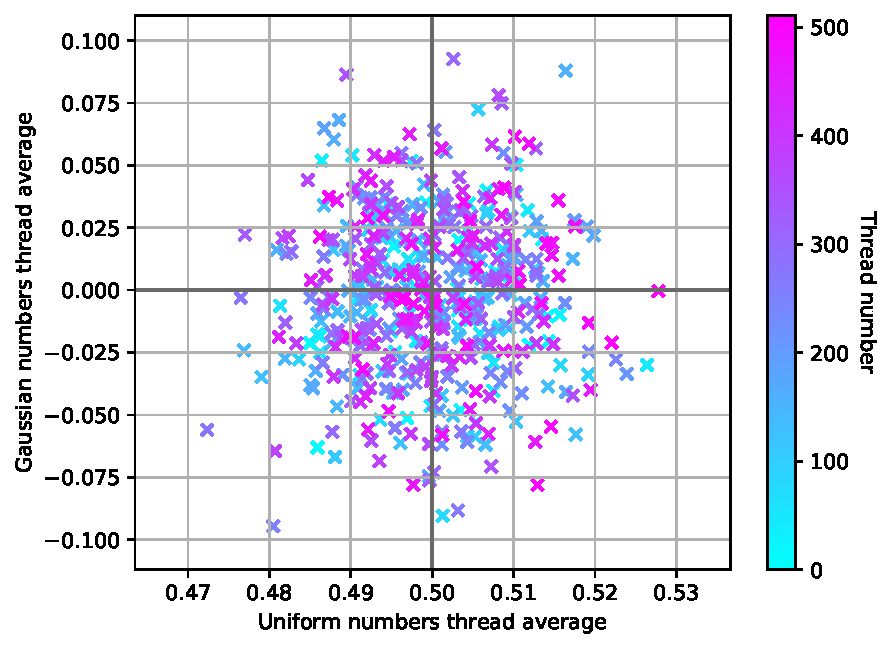
\includegraphics[scale=0.5]{graphs/CorrelationTests_UniAvgVsGaussAvg.pdf}
  \caption{}
  \label{fig:unigauss_avg}
\end{subfigure}%
\begin{subfigure}{.5\textwidth}
  \centering
  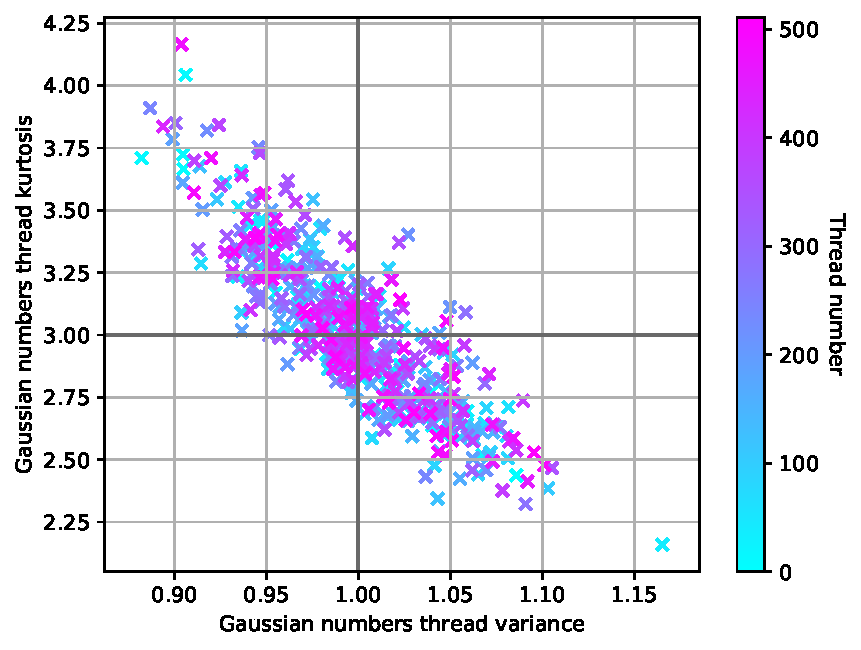
\includegraphics[scale=0.5]{graphs/CorrelationTests_KurtosisVsVariance.pdf}
  \caption{}
  \label{fig:variance_kurt}
\end{subfigure}
\caption{Dispersione di valori medi dei flussi di numeri pseudcasuali generati da ciascun \textit{thread} della GPU, il cui numero da 0 a 511 è indicato in scala cromatica da \textit{ciano} a \textit{magenta}. \textit{(a)} Dispersione delle medie dei numeri casuali generati nell'intervallo $[0,1]$ (ascissa) e dei numeri estratti da una distribuzione normale di media nulla e varianza unitaria (ordinata); \textit{(b)} dispersione di varianza e curtosi dei numeri estratti dalla medesima distribuzione normale di cui sopra. Le rette in \textit{grigio} evidenziano i valori teorici attesi per le quantità rappresentate: $\frac{1}{2}$ per la media di numeri uniformi, $0$, $1$ e $3$ per media, varianza e curtosi della distribuzione gaussiana.} 
\end{figure}

Per cominciare, in Figura \ref{fig:unigauss_avg} sono riportate le medie in ciascun \textit{thread} dei valori assunti dai numeri estratti uniformemente (in ascissa) e dai numeri estratti gaussianamente (in ordinata); come evidenziato dalla scala cromatica che indica il numero di \textit{thread}, la dispersione delle medie rispetto ai valori attesi indicati dalle rette in grigio non presenta asimmetrie significative. Un discorso analogo può essere fatto per la Figura \ref{fig:variance_kurt}, che riporta in ascissa la varianza
\begin{equation}
    \sigma^2 = \braket{{\left(r-\braket{r}\right)}^2}
    \label{eq:variance}
\end{equation}
e in ordinata la curtosi
\begin{equation}
    \text{Kurt}[r] = \frac{\braket{{\left(r-\braket{r}\right)}^4}}{\sigma^4}
    \label{eq:kurtosis}
\end{equation}
dei numeri generati gaussianamente, fatto salvo il \textit{caveat} che le due variabili sono evidentemente anticorrelate per la definizione di curtosi.

\begin{figure}[t]
\centering
\begin{subfigure}{.5\textwidth}
  \centering
  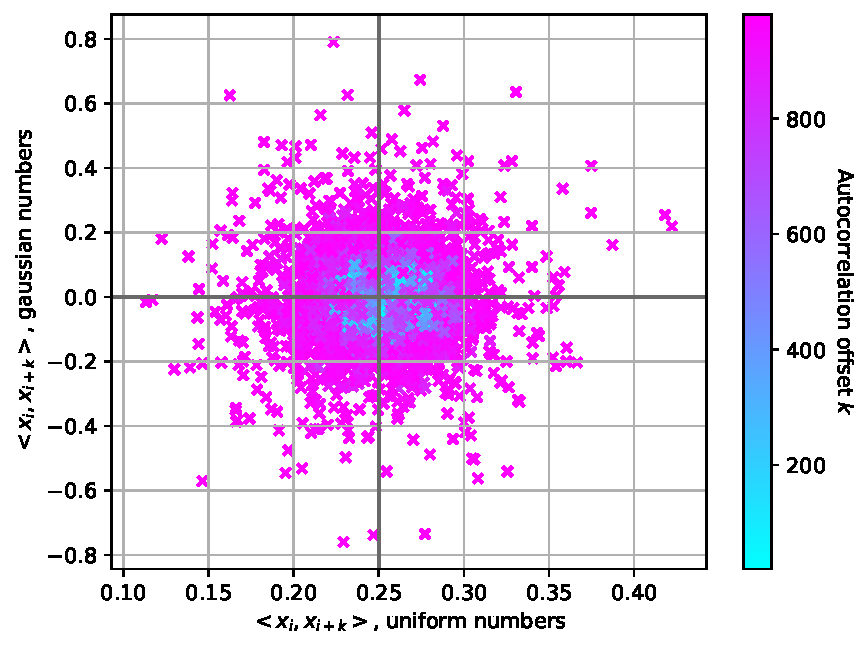
\includegraphics[scale=0.5]{graphs/CorrelationTests_IntraStreamCorrelations.pdf}
  \caption{}
  \label{fig:intra_corr}
\end{subfigure}%
\begin{subfigure}{.5\textwidth}
  \centering
  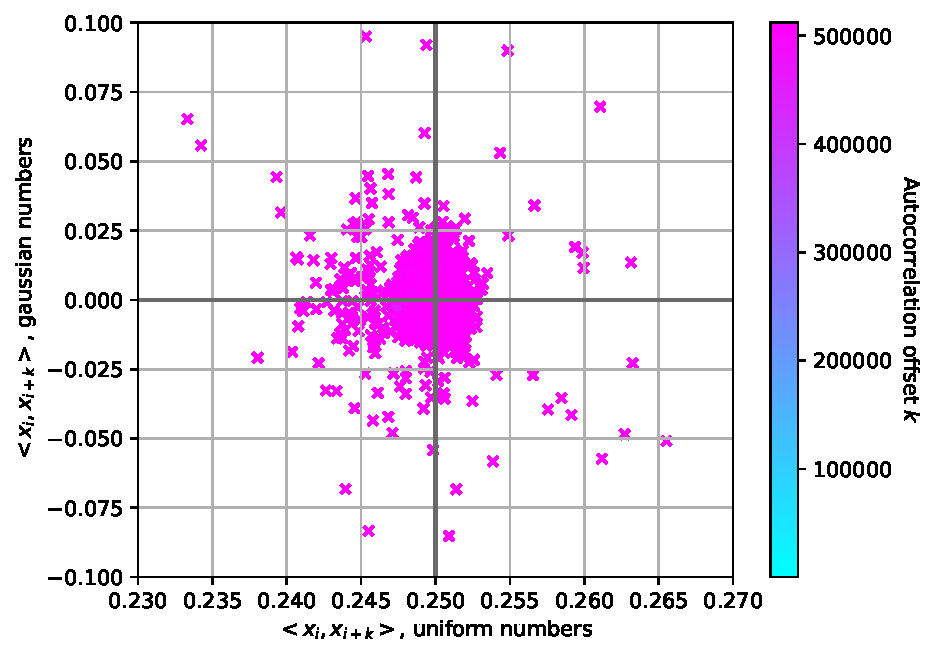
\includegraphics[scale=0.5]{graphs/CorrelationTests_InterStreamCorrelations.pdf}
  \caption{}
  \label{fig:inter_corr}
\end{subfigure}
\caption{Confronto tra autocorrelazioni $\braket{x_i x_{i+k}}$ nei casi di \textit{(a)} controllo \textit{intra-stream} sui flussi prodotti dai 512 \textit{thread}, e \textit{(b)} controllo \textit{inter-stream} effettuato su un singolo \textit{superstream} definito come in EQUAZIONE. In ascissa è riportata l'autocorrelazione nei flussi di numeri estratti uniformemente nell'intervallo $[0,1]$, in ordinata l'autocorrelazione dei numeri estratti secondo la distribuzione normale di media nulla e varianza unitaria; in scala cromatica da \textit{ciano} a \textit{magenta} è riportato il valore di $k$, mentre le rette in \textit{grigio} riportano i valori attesi ($\frac{1}{4}$ per la correlazione tra i numeri uniformi, $0$ per quella tra i numeri gaussiani).}
\end{figure}

Più spinoso è il caso della \textit{correlazione} $\braket{x_i x_{i+k}}$, dove $k$ è detto \textit{offset}. In Figura \ref{fig:intra_corr} è riportata la correlazione \textit{intra-stream} per i numeri distribuiti uniformemente (ascissa) e gaussianamente (ordinata). La scala cromatica questa volta indica l'\textit{offset} $k$, evidenziando come per $k$ elevati la dispersione dei risultati rispetto ai valori attesi (in grigio) sia fisiologicamente superiore in quanto sono disponibili meno numeri su cui effettuare la media. Ciononostante la distribuzione rimane visibilmente simmetrica e, pur non essendo evidenziati i risultati dei singoli \textit{thread}, studi in questa direzione non hanno evidenziato parzialità.

La Figura \ref{fig:inter_corr} riporta risultati secondo il medesimo schema della precedente applicati a un <<\textit{super-stream}>> ottenuto combinando tutti i 512 \textit{thread} secondo la formula
\begin{equation}
    w_{k=iN+j} = r_j^i,
    \label{eq:superstream}
\end{equation}
dove $j=1,...,512$ è l'indice di \textit{thread} e $i=1,...,1000$ è l'indice di numero generato. Se i numeri gaussiani preservano una distribuzione simmetrica intorno alla correlazione attesa, in quelli gaussiani spicca una polarizzazione a favore di valori leggermente inferiori a $\frac{1}{4}$.

\begin{figure}[t]
\centering
\begin{subfigure}{.5\textwidth}
  \centering
  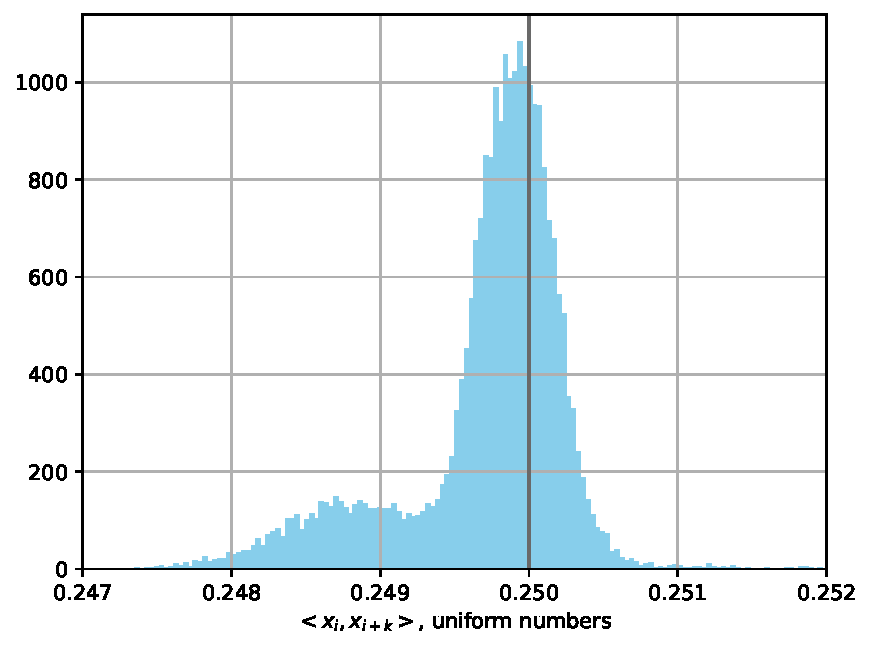
\includegraphics[scale=0.5]{graphs/CorrelationTests_UniformInterStreamAutocorrelationHistogram.pdf}
  \caption{}
  \label{fig:inter_uni_autocorr_histo}
\end{subfigure}%
\begin{subfigure}{.5\textwidth}
  \centering
  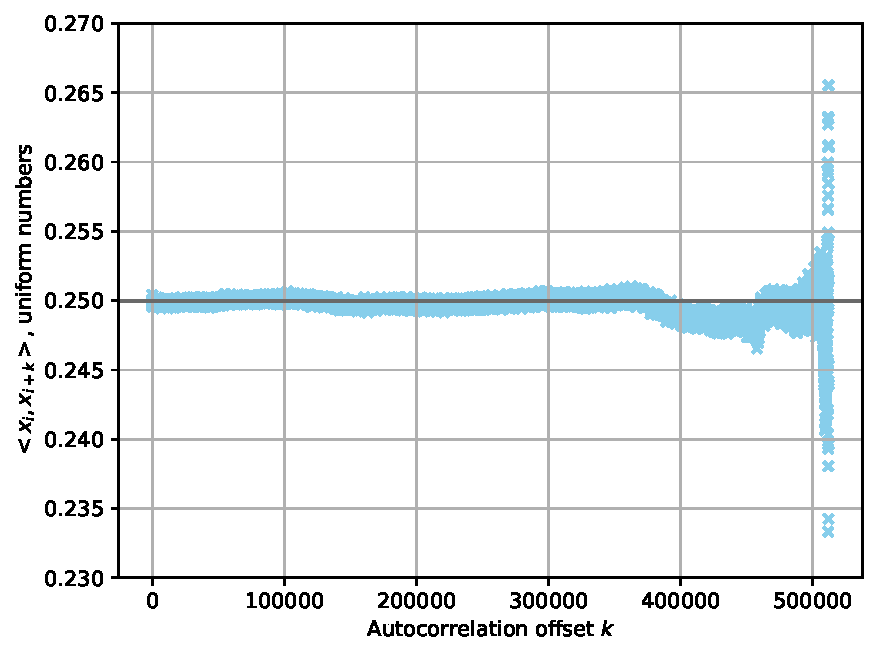
\includegraphics[scale=0.5]{graphs/CorrelationTests_UniformInterStreamAutocorrelationVsOffset.pdf}
  \caption{}
  \label{fig:inter_uni_autocorr_offset}
\end{subfigure}
\caption{\textit{(a)} Istogramma delle autocorrelazioni $\braket{x_i x_{i+k}}$ \textit{inter-stream} del flusso di numeri pseudocasuali estratti uniformemente nell'intervallo $[0,1]$; \textit{(b)} andamento delle correlazioni in funzione dell'\textit{offset} $k$.}
\end{figure}

Per indagare più a fondo questa distorsione abbiamo riportato in Figura \ref{fig:inter_uni_autocorr_histo} un istogramma delle correlazioni \textit{inter-stream} dei numeri uniformi e in Figura \ref{fig:inter_uni_autocorr_offset} il suo andamento in funzione di $k$. Da questi grafici è evidente come il picco secondario appaia per \textit{offset} particolarmente alti; ciononostante, anche l'andamento prima dell'anomalia presenta una forma vagamente oscillatoria, evidenziando come il flusso di numeri pseudocasuali non soddisfi pienamente la richiesta di autoindipendenza.

\begin{figure}[t]
\centering
\begin{subfigure}{.5\textwidth}
  \centering
  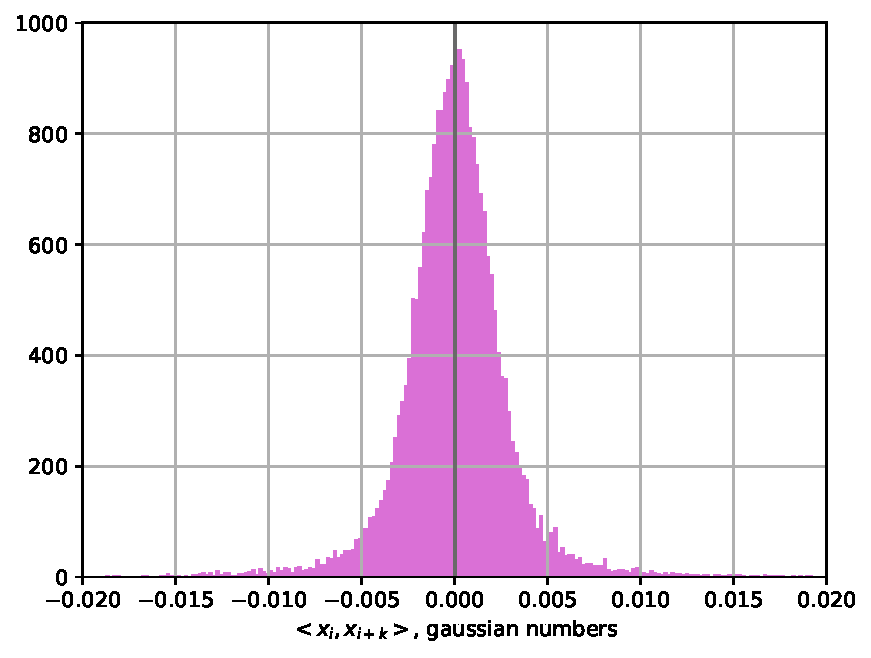
\includegraphics[scale=0.5]{graphs/CorrelationTests_GaussInterStreamAutocorrelationHistogram.pdf}
  \caption{}
  \label{fig:inter_gauss_autocorr_histo}
\end{subfigure}%
\begin{subfigure}{.5\textwidth}
  \centering
  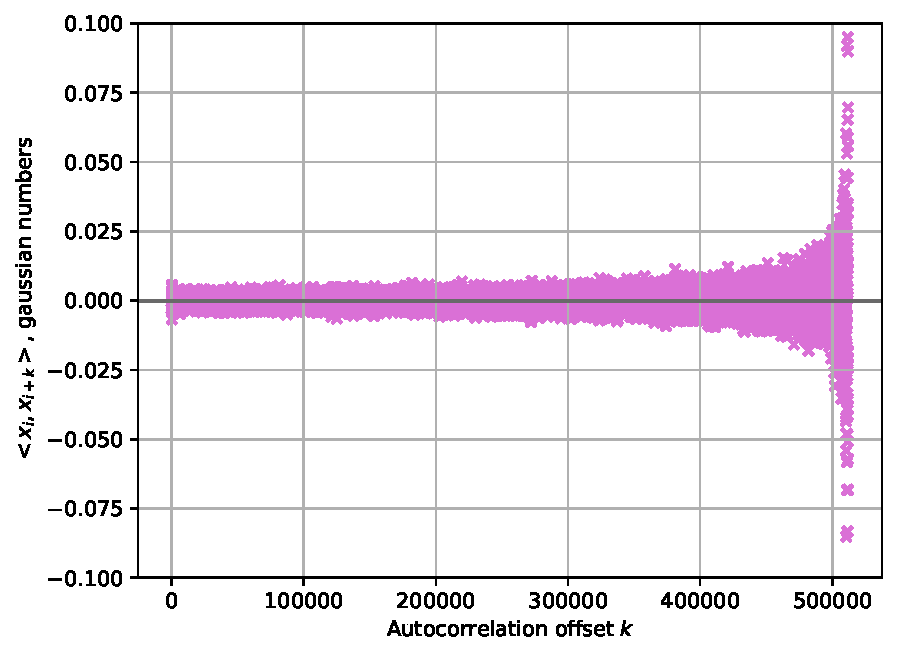
\includegraphics[scale=0.5]{graphs/CorrelationTests_GaussInterStreamAutocorrelationVsOffset.pdf}
  \caption{}
  \label{fig:inter_gauss_autocorr_offset}
\end{subfigure}
\caption{\textit{(a)} Istogramma delle autocorrelazioni $\braket{x_i x_{i+k}}$ \textit{inter-stream} del flusso di numeri pseudocasuali estratti uniformemente secondo una distribuzione normale di media nulla e varianza unitaria; \textit{(b)} andamento delle correlazioni in funzione dell'\textit{offset} $k$.}
\end{figure}

Ciononostante, le analoghe Figure \ref{fig:inter_gauss_autocorr_histo} e \ref{fig:inter_gauss_autocorr_offset} evidenziano come, pur essendo i numeri gaussiani generati a partire da quelli uniformi, in essi sia essenzialmente assente ogni spettro di autocorrelazione. Poiché le variabili gaussiane sono quelle di reale interesse, i controlli effettuati avvalorano l'indipendenza e l'affidabilità delle nostre simulazioni.

\section{(B-3) \textit{Pricing} dell'opzione \textit{performance corridor}}
\subsection{(B-3-a) Dipendenza dalle date di rilevamento e dal numero di simulazioni}

\begin{figure}[t]
    \centering
    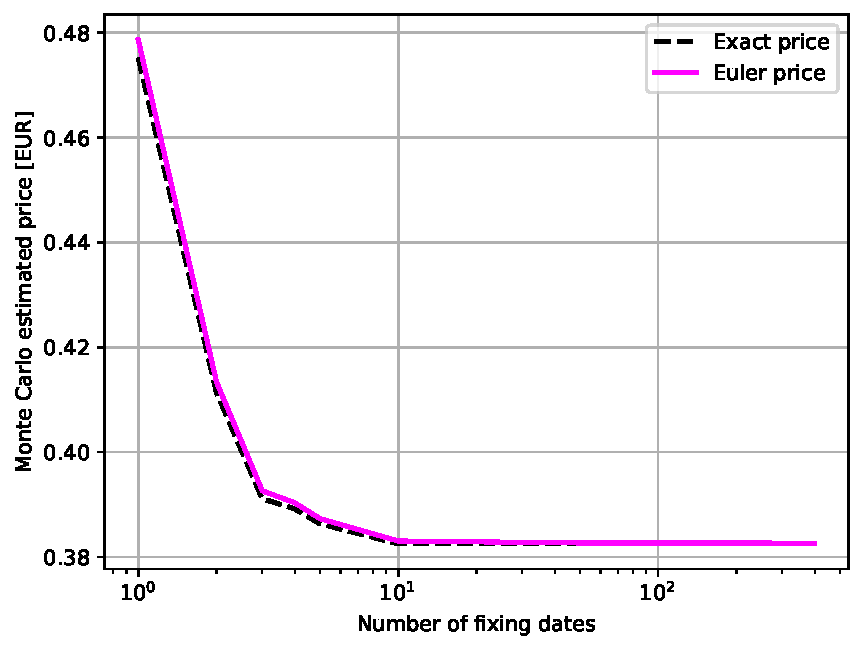
\includegraphics[scale=0.5]{graphs/OptionPriceVsM_PriceVsM_N100mln.pdf}
    \caption{Confronto dell'andamento del prezzo dell'opzione \textit{performance corridor} in funzione del numero di date di rilevamento calcolato secondo lo schema di Eulero (\textit{magenta}) e secondo lo schema esatto (\textit{nero}, \textit{tratteggiato}).}
    \label{fig:exactvseuler_M}
\end{figure}

\begin{figure}[t]
    \centering
    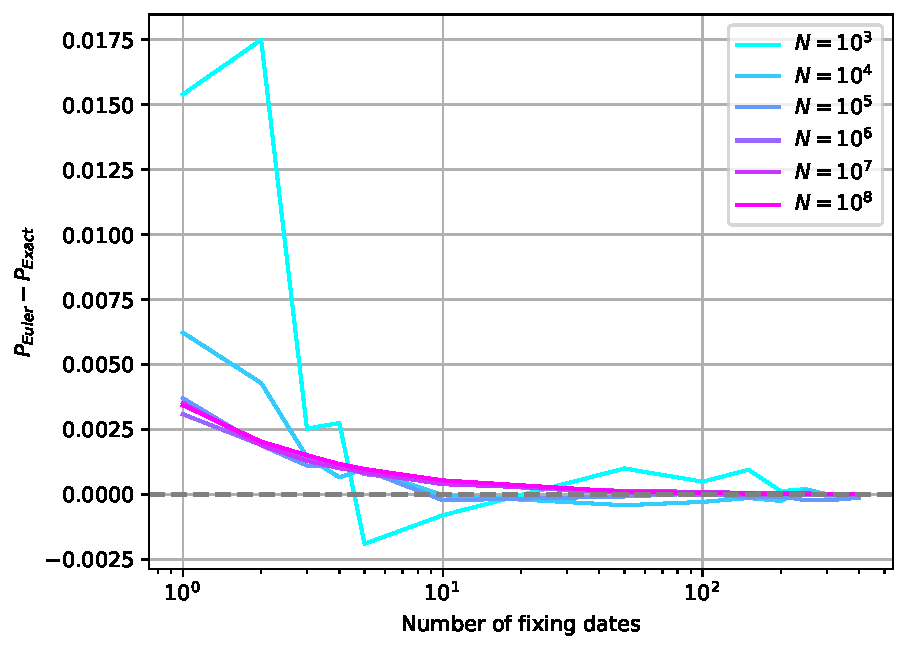
\includegraphics[scale=0.5]{graphs/OptionPriceVsM_DiscrepancyVsM_WithDifferentNs.pdf}
    \caption{Differenza tra i prezzi dell'opzione \textit{performance corridor} calcolati secondo lo schema di Eulero e secondo lo schema esatto in funzione del numero di date di rilevamento; da \textit{ciano} a \textit{magenta} curve con numero crescente di simulazioni da ${10}^3$ a ${10}^8$, in \textit{grigio tratteggiato} il valore asintotico di discrepanza nulla.}
    \label{fig:ex_eul_discrep_M}
\end{figure}

\lipsum[1-3]

\subsection{(B-3-b) Dipendenza dal valore di $B$}

\begin{figure}[t]
    \centering
    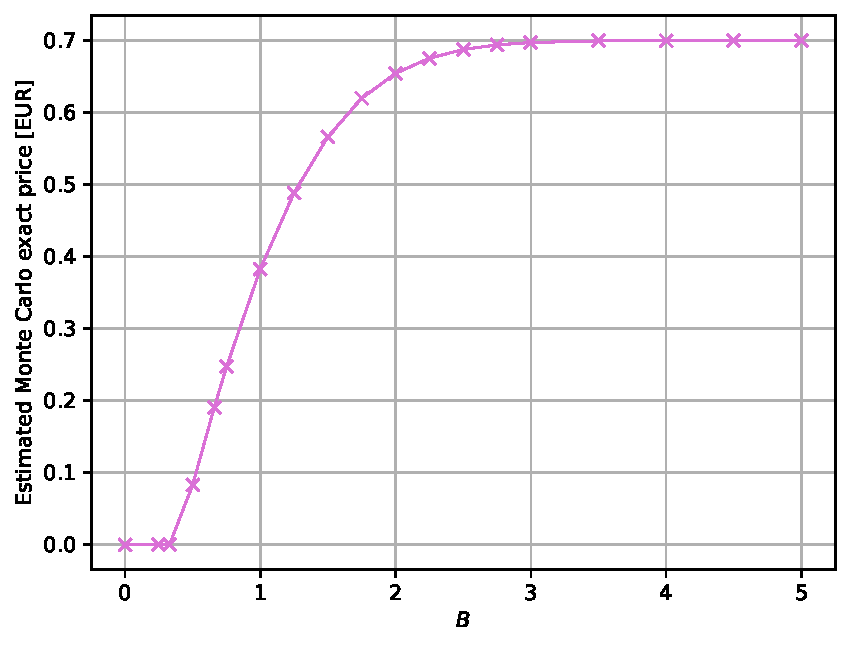
\includegraphics[scale=0.5]{graphs/OptionPriceVsB_PriceVsB_N200mln.pdf}
    \caption{Andamento del prezzo dell'opzione \textit{performance corridor} stimato secondo lo schema esatto in funzione del parametro $B$ che determina l'altezza della barriera.}
    \label{fig:price_vs_b}
\end{figure}

\lipsum[1-3]


\section{(B-4) Studi sull'errore Monte Carlo}
\subsection{(B-4-a) Dipendenza dalle date di rilevamento e dal numero di simulazioni}

\begin{figure}[t]
\centering
\begin{subfigure}{.5\textwidth}
  \centering
  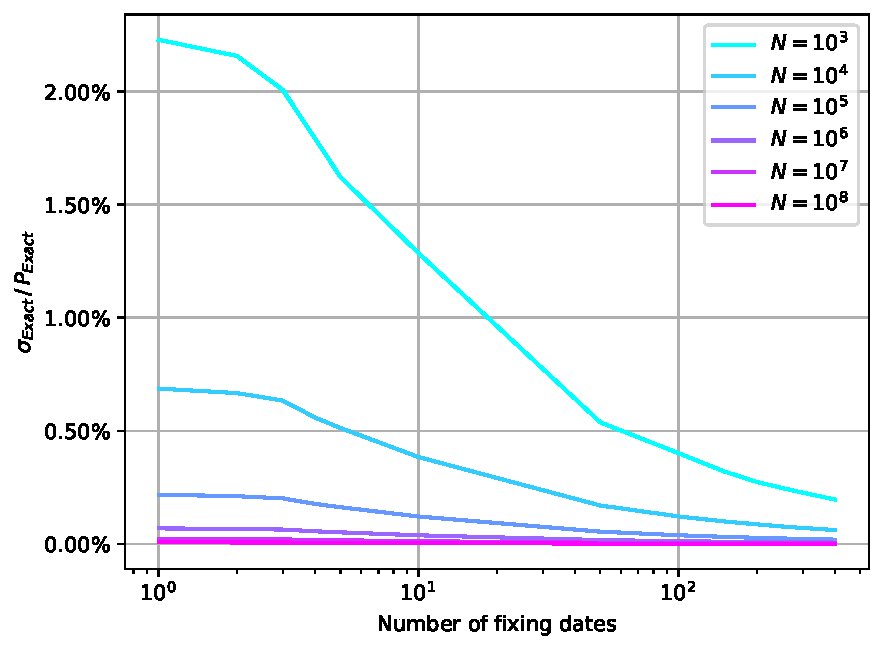
\includegraphics[scale=0.5]{graphs/OptionPriceVsM_ExactErrorVsM_WithDifferentNs.pdf}
  \caption{}
  \label{fig:exact_error_M}
\end{subfigure}%
\begin{subfigure}{.5\textwidth}
  \centering
  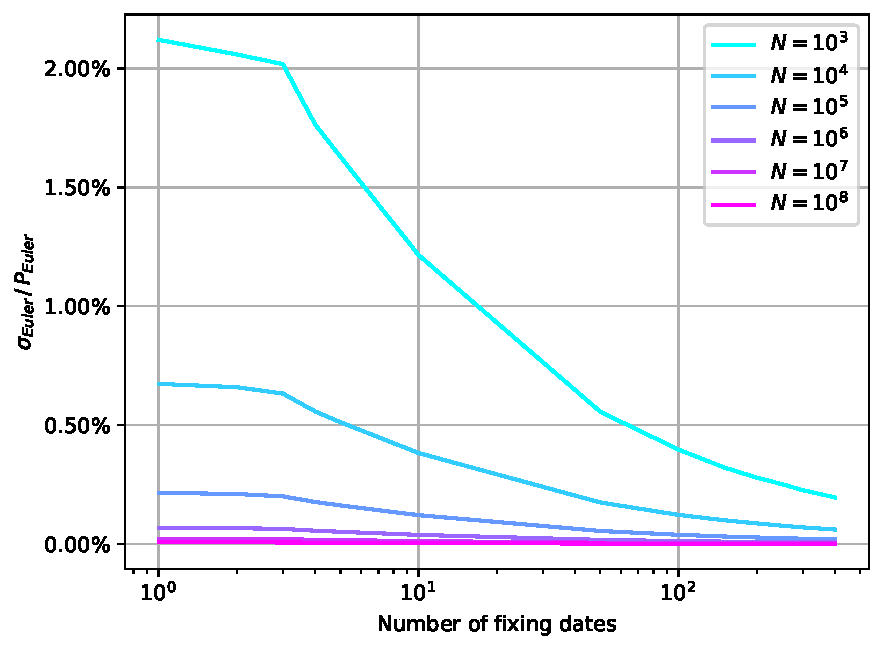
\includegraphics[scale=0.5]{graphs/OptionPriceVsM_EulerErrorVsM_WithDifferentNs.pdf}
  \caption{}
  \label{fig:euler_error_M}
\end{subfigure}
\caption{Andamento dell'errore relativo Monte Carlo in funzione del numero di date di rilevamento rispetto al prezzo calcolato \textit{(a)} secondo lo schema esatto e \textit{(b)} secondo lo schema di Eulero; curve di colore da \textit{ciano} a \textit{magenta} corrispondono a un numero crescente di simulazioni da ${10}^3$ a ${10}^8$.}
\end{figure}

\lipsum[1-3]

\subsection{(B-4-b) Dipendenza dal valore di $B$}

\begin{figure}[t]
    \centering
    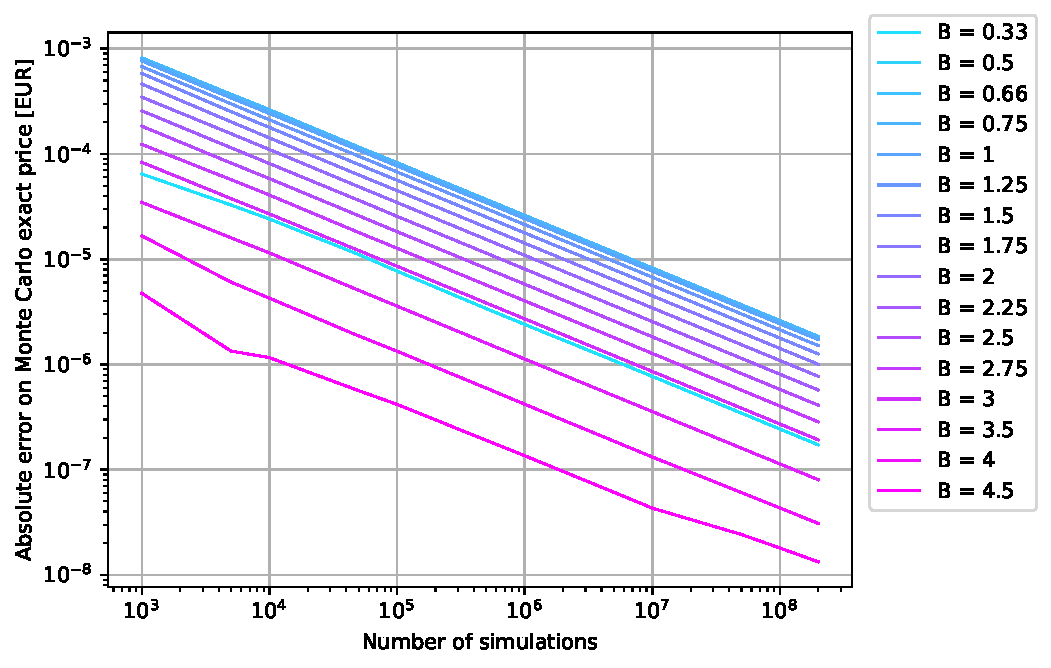
\includegraphics[scale=0.5]{graphs/OptionPriceVsB_ExactErrorVsN_WithAllBs.pdf}
    \caption{Errore assoluto Monte Carlo rispetto al prezzo calcolato secondo lo schema esatto in funzione del numero di simulazioni effettuate; curve di colore da \textit{ciano} a \textit{magenta} corrispondono a valori crescenti del parametro $B$.}
    \label{fig:error_vs_B}
\end{figure}

\begin{figure}[t]
    \centering
    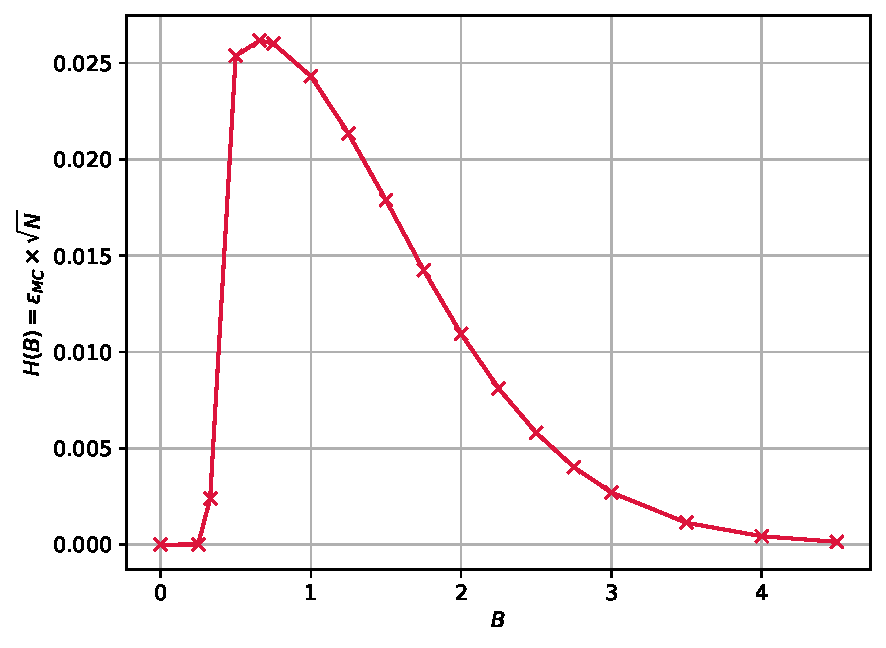
\includegraphics[scale=0.5]{graphs/OptionPriceVsB_HBVsB.pdf}
    \caption{Andamento del valore della costante moltiplicativa $H(B)$ dell'EQUAZIONE in funzione di $B$.}
    \label{fig:HB_vs_B}
\end{figure}

\lipsum[1-3]


\section{(B-5) Studi sui tempi di esecuzione} \label{sec:comptime}
\subsection{(B-5-a) Analisi dei tempi di esecuzione in GPU}
\begin{figure}[t]
    \centering
    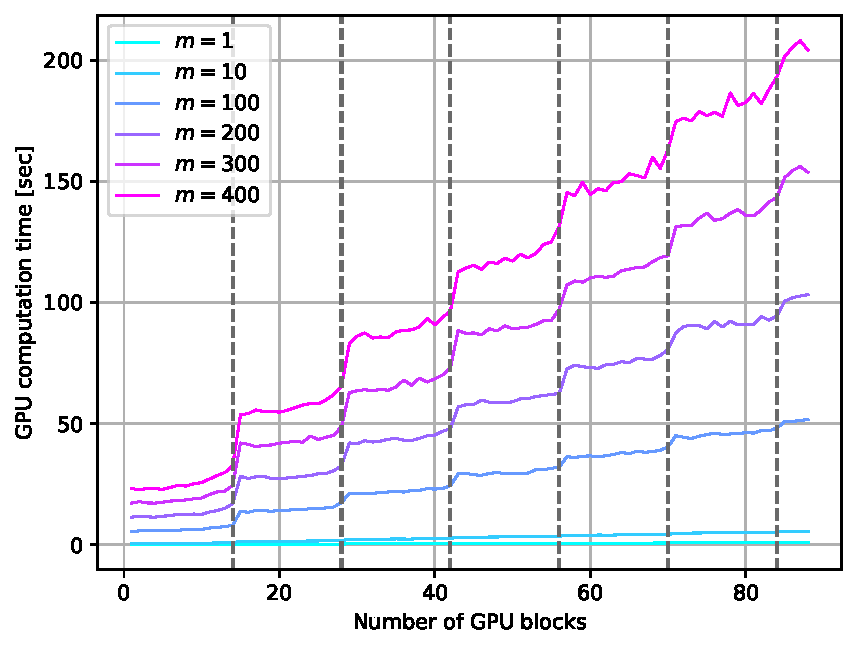
\includegraphics[scale=0.5]{graphs/ComputationTime_Tesla_GPUTimeVsNOfBlocks_VariousM_1000SimsPerThread.pdf}
    \caption{Tempi di esecuzione dell'algoritmo su GPU al crescere del numero di blocchi per diverse densità di date di rilevamento. Nelle simulazioni cronometrate in ogni blocco erano istanziati 512 \textit{thread}, ciascuno incaricato di eseguire 1000 simulazioni dell'evoluzione del prezzo del sottostante.}
    \label{fig:gpucomptime}
\end{figure}
\lipsum[1-3]

\subsection{(B-5-b) Analisi del fattore di guadagno GPU-CPU}
\lipsum[1-3]

\section{(B-6) Limiti di applicabilità e approssimazioni} \label{sec:limits}

\begin{figure}[t]
    \centering
    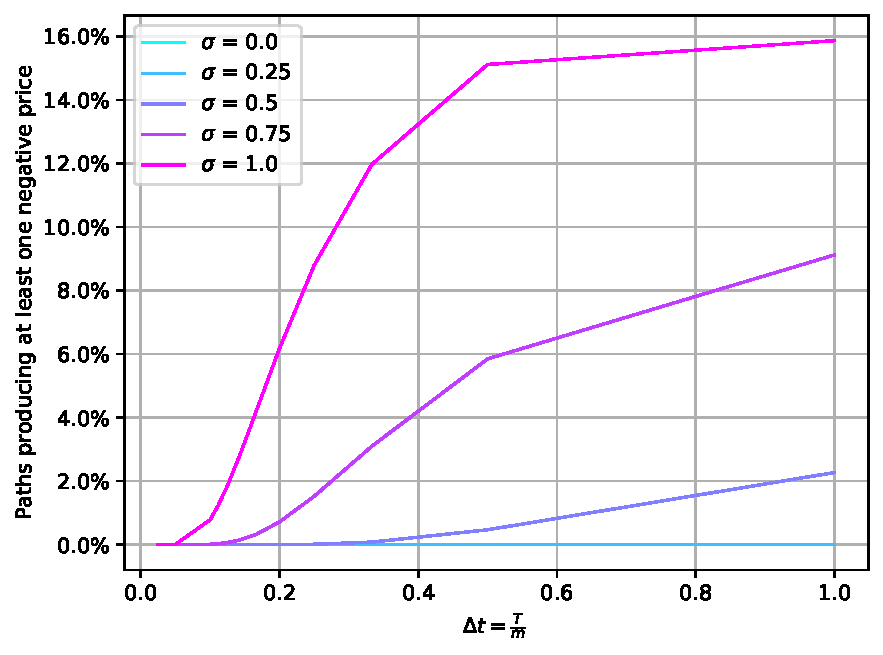
\includegraphics[scale=0.5]{graphs/NegativePrices_PercentageVsM_VariousSigmas.pdf}
    \caption{Percentuale di evoluzioni simulate del prezzo del sottostante che riportano almeno un'istanza di prezzo $S(t_i)$ negativo al variare della distanza temporale $\Delta t$ tra le date di rilevamento; curve di colore da \textit{ciano} a \textit{magenta} corrispondono a valori crescenti della volatilità $\sigma$ del mercato.}
    \label{fig:negativeprices}
\end{figure}
\lipsum[1-3]